\part{Dataset Labelling}
%%%%%%%%%%%%%%%%%%%%%%%%%%%%%%%%%%%%%%%%%%%%%%%%%%%%%%%%%%%%%%%%%%%%%%%%%
% Dataset Labelling                                                     %
%%%%%%%%%%%%%%%%%%%%%%%%%%%%%%%%%%%%%%%%%%%%%%%%%%%%%%%%%%%%%%%%%%%%%%%%%
\section{Motivation and background}
This project is intimately linked with the neural networks project, but since a lot of time has been dedicated towards it, it merits a section for itself. This project is aimed at tackling the issue of lack of data, by providing a mechanism to get more data easily. The current bottleneck in aquiring more data is labelling the data, it's conceivably easy to set up a system to video hand washing, but to label it requires a bespoke system.

%%%%%%%%%%%%%%%%%%%%%%%%%%%%%%%%%%%%%%%%%%%%%%%%%%%%%%%%%%%%%%%%%%%%%%%%%
% Overview                                                              %
%%%%%%%%%%%%%%%%%%%%%%%%%%%%%%%%%%%%%%%%%%%%%%%%%%%%%%%%%%%%%%%%%%%%%%%%%
\section{Overview}
The process of labelling the data is divided into three distinct stages, first preprocessing to prepare the data for labelling, then the actual labelling of the data, and then comparison of the labelled data between differant people.
    \subsection{Preprocessing}
    The data is captured on an Intel Realsense camera, which saves the data in ROS-bag format which is an uncompressed video \cite{intelrosbag}. This needs to be converted into an ordinary video format (such as MPEG-4 \cite{wiegand2003overview}). There is a tool within the library of the Realsense camera which converts to still images, so another tool called FFMPEG \cite{ffmpeg} is used to convert to MPEG-4. This entire process is done with in a bash script, so the end user only needs to provide the ROS-bag file as an argument to the script and it will output a video that can be used for labelling.
    \subsection{Labelling}
    The data is labelled in a GUI web app. The programme is started from a terminal and then the labelling is done in a HTML5 application which allows the user to label the class for each frame of the video, as well as the Region Of Interest, hereby ROI. The output is saved to a text file, the markup file.

    \begin{figure}[h]
        \centering
        \fbox{ 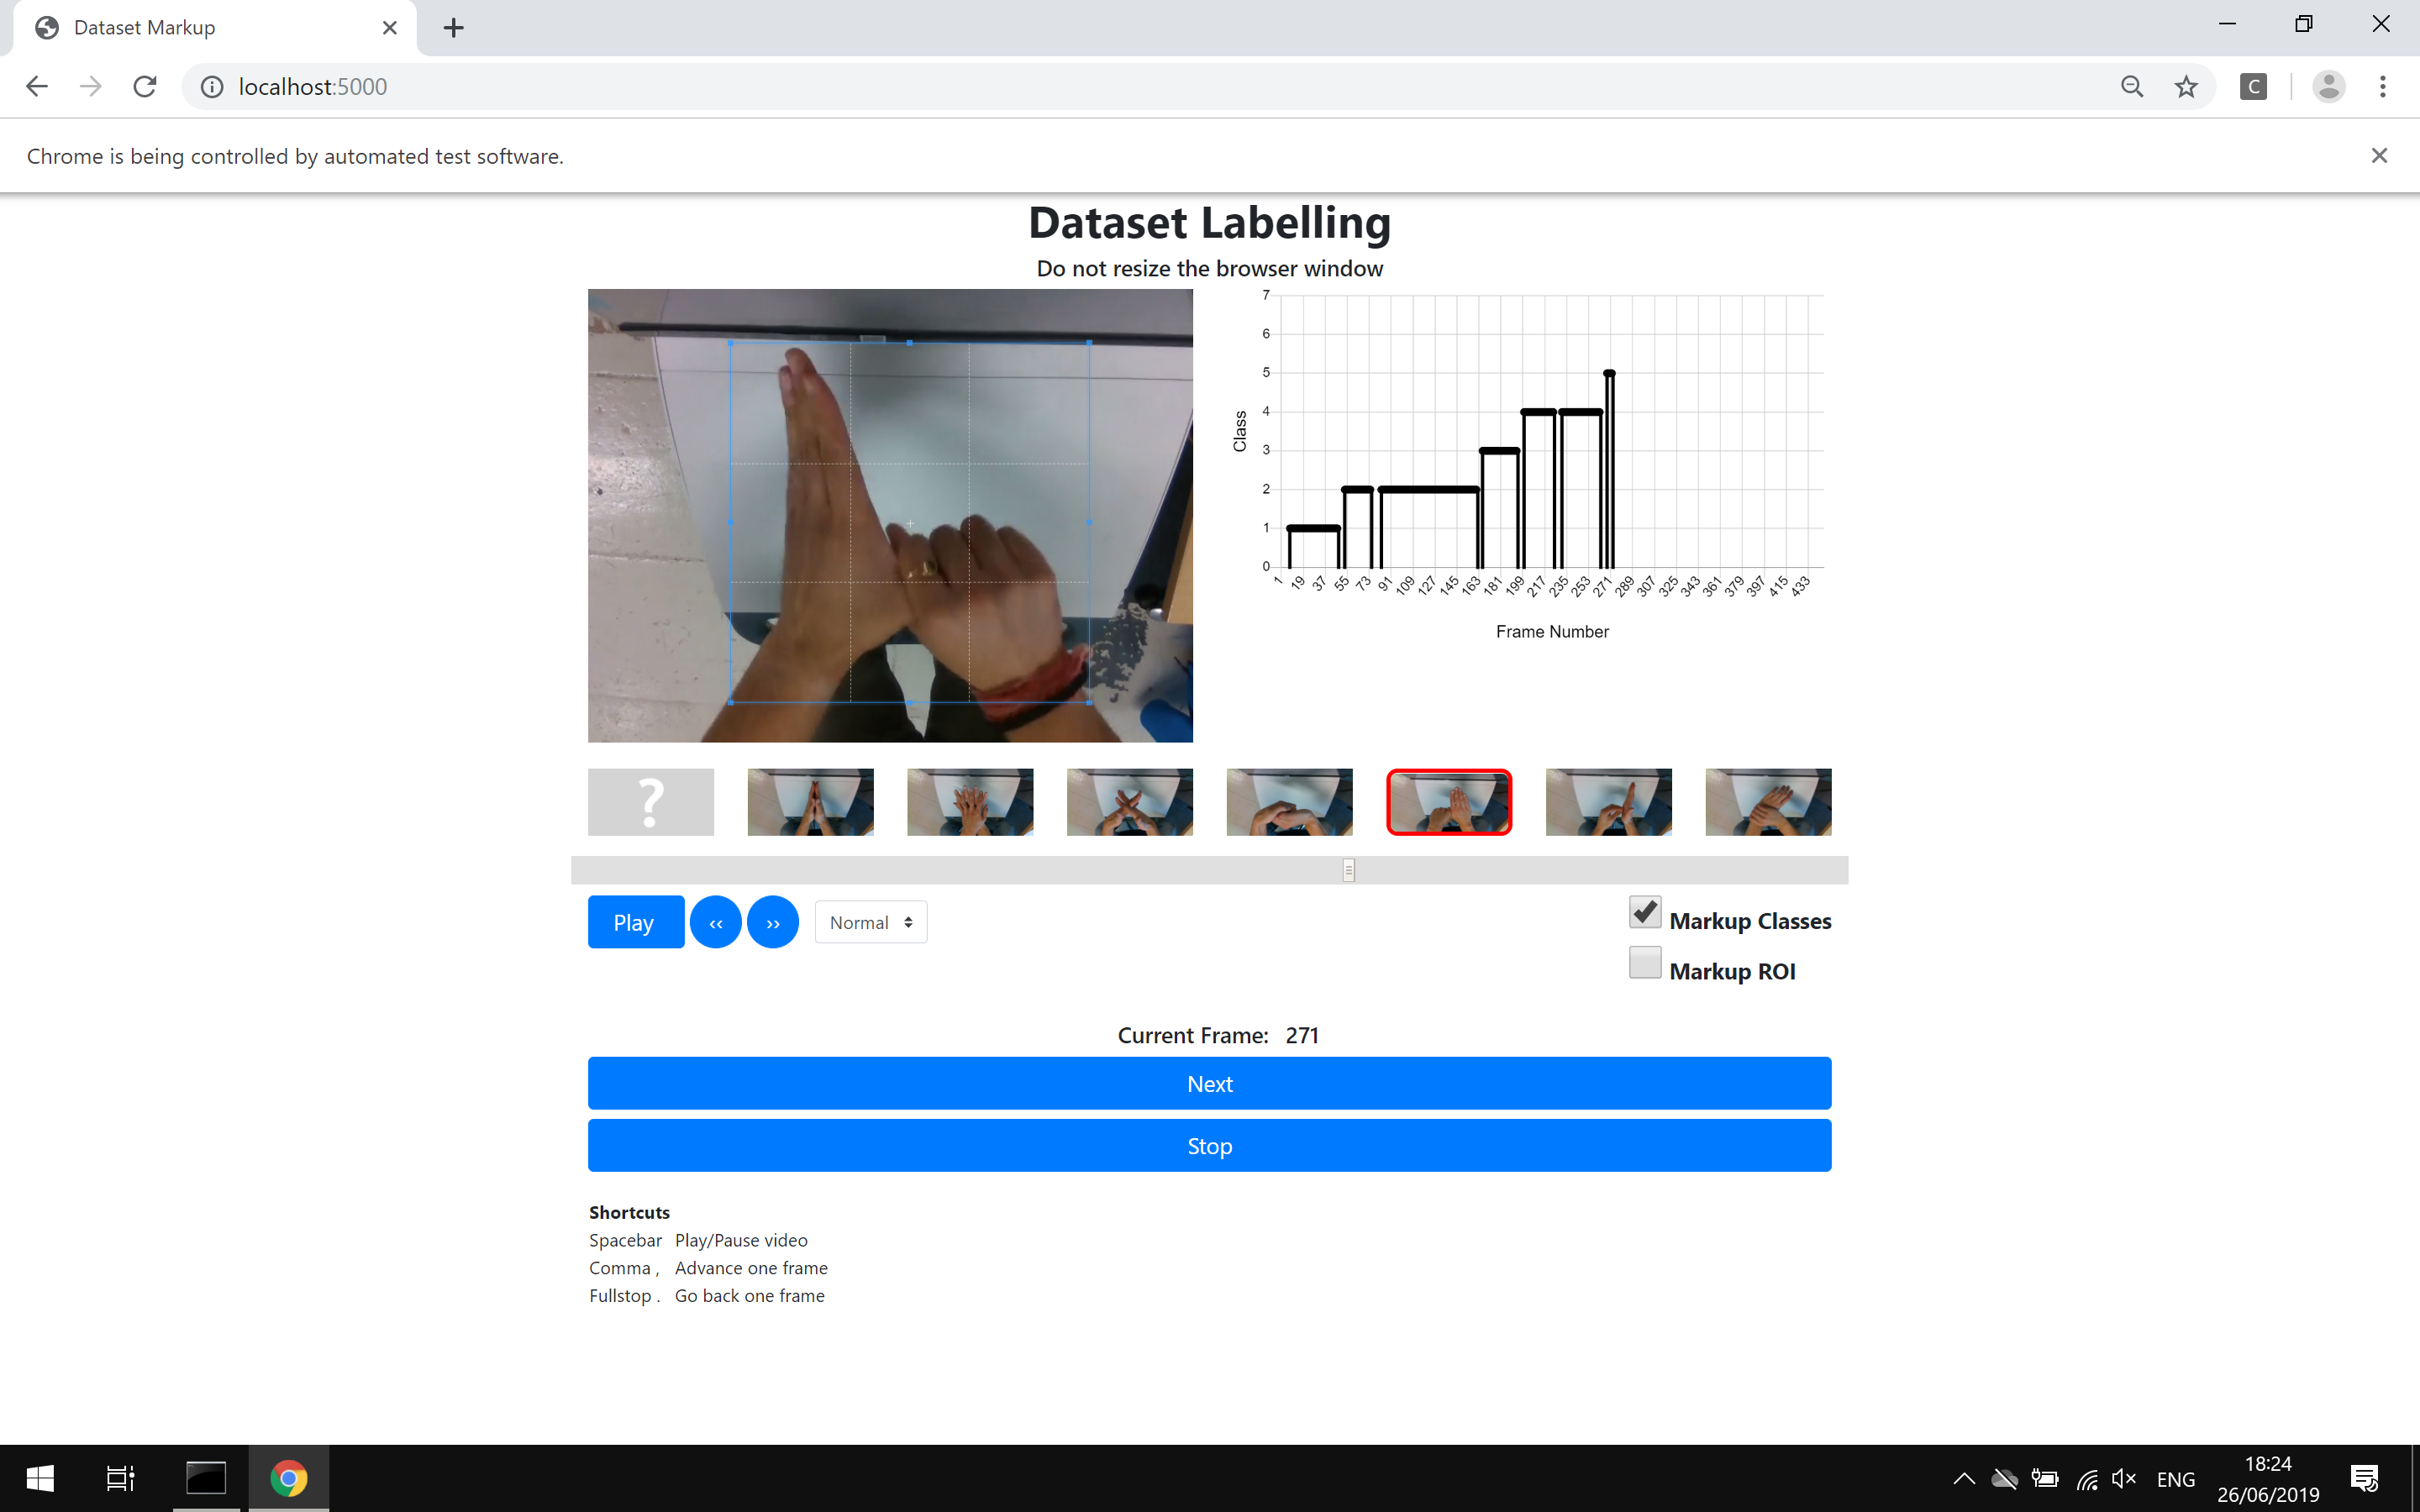
\includegraphics[width=450px]{../img/markup_screenshot.png} }
        \caption{Screenshot of the labelling web app, all images are \copyright \space Glanta Ltd.}
        \label{fig:markupscreenshot}
    \end{figure}

    \subsection{Comparison} 
    It is likely that at least some errors will be made in the labelling step, therefore this step will assume that at least two differant people performed labelling on the same video, or at least the same person did the labelling twice. A programme was written that will compare two differant markup files, and it will report where there was disagreements between two markup files so that they can be looked at again.

%%%%%%%%%%%%%%%%%%%%%%%%%%%%%%%%%%%%%%%%%%%%%%%%%%%%%%%%%%%%%%%%%%%%%%%%%
% Technical details                                                     %
%%%%%%%%%%%%%%%%%%%%%%%%%%%%%%%%%%%%%%%%%%%%%%%%%%%%%%%%%%%%%%%%%%%%%%%%%
\section{Technical Details}
    \subsection{Labelling}
    Since the app is a web app, the code is divided into two parts, the server code, and the client code. The layout of the output file is as follows:

    \[
    \begin{bmatrix}
    x_{10} & y_{10} & x_{20} & y_{20} & c_{0} \\
    x_{11} & y_{11} & x_{21} & y_{21} & c_{1} \\
    x_{12} & y_{12} & x_{22} & y_{22} & c_{2} \\
    x_{13} & y_{13} & x_{23} & y_{23} & c_{3} \\
    \vdots & \vdots & \vdots & \vdots & \vdots\\
    x_{1n} & y_{1n} & x_{2n} & y_{2n} & c_{n} 
    \end{bmatrix}
    \]
    \begin{gather*}
    x, y \in \mathbb{R} [0, 1]\\
    c \in \mathbb{Z}
    \end{gather*}

    The $x$ and $y$ values represent coordinates describing an ROI box (top left, and bottom right), and the $c$ value represents the class (the classes must be encoded in integer form). Each row represents one frame. By default, all values are set to -1 to denote that they have either not been labelled, or are 'ambiguous'. The coordinates represent the ROI in a proportional system, so if the image is 350 pixels wide, and a $y$ coordinate was $0.22$, then that would refer to the 77th pixel. The coordinates are represented proportionally because the original video is scaled from the original BAG file, and since the ROI box does not have to be precisely correct, this system is acceptable in my opinion. In the markup file, the $x$ and $y$ values are represented by floating point values, and the class values are signed integers.

        \subsubsection{Server Code}
        This is primarily a Flask app \cite{flaskpocoo}. Flask is a Python web framework, similar in concept to Django but without the model layer, and web security features, which are not necesasary for this application. It is thus easier to write an application in Flask as opposed to Django. The server code is divided into two main areas, the view, and the template. The server acts 'dumb', its main task apart from serving the client application initially is to take the marked up data and save it, it does not do any processing with the data itself. The view exposes a HTTP GET, and HTTP POST method for downloading, and uploading the markup data.

        \subsubsection{Client Code}
        All of the logic for marking up the data happens in the client code, and since this is a web application, all of this code is written in JavaScript. The results are stored in an array of arrays. Each entry in the parent array corresponds to a frame, and each array in that corresponds to the coordinates, and class for that frame. Every time the video is played, paused, its frame put forward, or backward, it triggers a method to push the array back to the server using a Jquery AJAX method.

            \paragraph{Classes}
            The class is marked simply by pressing a button for what the class is for the currently displayed frame. The currently displayed frame is obtained with the following function:
                \begin{lstlisting}[style=JSStyle]
function return_current_frame() {
    var curr_frame = Math.floor(theVideo.currentTime*frameRate);
    if(curr_frame >= frame_count) {
        curr_frame = frame_count - 1;
    }
    return curr_frame;
}
            \end{lstlisting} 
            Since HTML5 video does not expose a way to get the frame number directly, it has to be obtained by multiplying the current time by the frame rate. Since there also is no way of determening the frame rate directly, a server-side HTTP GET method is used which uses ffprobe to determine the frame rate and push that to the client side using a Jquery AJAX method.

            \paragraph{ROI}
            Finding a way to mark ROI from a web browser is more difficult, since there weren't any out of the box solutions that existedas far as I could tell. The solution involved using a Javascript library called Cropper.js \cite{cropperjs}. This library is designed to load an image in for marking an area to crop. It was adapted to this solution by overlaying it on the video, and every time the video frame changed, the current cropped coordinates were obtained and saved to the results matrix. The method of overlaying led to issues with the coordinates that it outputted did not correspond to the video resolution due to the nature of this solution. The $x$ coordinates ranged from 0, to the width of the HTML5 canvas element, which means that this can be converted to proportional coordinates (mentioned above) easily. The $y$ coordinates on the other hand presented more issues, since they ranged from approximately $[-9.44, 159.31]$, and I could not source a reasonable explanation as to why this was the case. This quirk was consistent across browers and operating systems, so the $y$ coordinates were converted to proportional coordinates by fitting them to a line with $y=mx+c$ using the coordinates $(-9.44,0)$ and $(159.31,1)$. To prevent edge cases straying above 1, or below zero, the output values were clamped between these two values. The final code to do the conversion looks like the following:

            \begin{lstlisting}[style=JSStyle]
function get_proportional_coordinates(cropper_instance, x1_func, y1_func, x2_func, y2_func) {
    var curr_width = cropper_instance.getCanvasData().naturalWidth;
    var y1_proportional = (y1_func * (4/675)) + (944/16875);
    var y2_proportional = (y2_func * (4/675)) + (944/16875);
    var x1_proportional = x1_func / curr_width;
    var x2_proportional = x2_func / curr_width;

    if      (y1_proportional > 1)   y1_proportional = 1;
    else if (y1_proportional < 0)   y1_proportional = 0;

    if      (y2_proportional > 1)   y2_proportional = 1;
    else if (y2_proportional < 0)   y2_proportional = 0;

    if      (x1_proportional > 1)   x1_proportional = 1;
    else if (x1_proportional < 0)   x1_proportional = 0;

    if      (x2_proportional > 1)   x2_proportional = 1;
    else if (x2_proportional < 0)   x2_proportional = 0;
    
    return {
        x1_proportional: x1_proportional,
        y1_proportional: y1_proportional,
        x2_proportional: x2_proportional,
        y2_proportional: y2_proportional,
    }
}
    \end{lstlisting} 

    \subsection{Comparison}
    Two differant markups of the same video are compared with a Python script. The task is divided into two parts, one camparing the class markup, and one comparing the class markup. The inputs are treated as signals, and processed to produce a sin